\documentclass[12pt]{beamer}
\usepackage{amsmath}
\usepackage{mathtools}
\usepackage{multimedia}
\usepackage{hyperref}
\usepackage{booktabs}

\usefonttheme{professionalfonts} % using non standard fonts for beamer
\usefonttheme{serif} % default family is serif
%\documentclass[12pt]{beamerthemeSam.sty}
\usepackage{epsf}
%\usepackage{pstricks}
%\usepackage[orientation=portrait,size=A4]{beamerposter}
\geometry{paperwidth=160mm,paperheight=120mm}
%DT favorite definitions
\def\LL{\left\langle}	% left angle bracket
\def\RR{\right\rangle}	% right angle bracket
\def\LP{\left(}		% left parenthesis
\def\RP{\right)}	% right parenthesis
\def\LB{\left\{}	% left curly bracket
\def\RB{\right\}}	% right curly bracket
\def\PAR#1#2{ {{\partial #1}\over{\partial #2}} }
\def\PARTWO#1#2{ {{\partial^2 #1}\over{\partial #2}^2} }
\def\PARTWOMIX#1#2#3{ {{\partial^2 #1}\over{\partial #2 \partial #3}} }

\def\rightpartial{{\overrightarrow\partial}}
\def\leftpartial{{\overleftarrow\partial}}
\def\diffpartial{\buildrel\leftrightarrow\over\partial}

\def\BC{\begin{center}}
\def\EC{\end{center}}
\def\BN{\begin{enumerate}}
\def\EN{\end{enumerate}}
\def\BI{\begin{itemize}}
\def\EI{\end{itemize}}
\def\BE{\begin{displaymath}}
\def\EE{\end{displaymath}}
\def\BEA{\begin{eqnarray*}}
\def\EEA{\end{eqnarray*}}
\def\BNEA{\begin{eqnarray}}
\def\ENEA{\end{eqnarray}}
\def\EL{\nonumber\\}

\newcommand{\BCC}{\begin{columns}}
\newcommand{\ECC}{\end{columns}}
\newcommand{\HC}{\column{0.5\textwidth}}
\newcommand{\etal}{{\it et al.}}
\newcommand{\gbeta}{6/g^2}
\newcommand{\la}[1]{\label{#1}}
\newcommand{\ie}{{\em i.e.\ }}
\newcommand{\eg}{{\em e.\,g.\ }}
\newcommand{\cf}{cf.\ }
\newcommand{\BS}{\bigskip}
\newcommand{\etc}{etc.\ }
\newcommand{\atantwo}{{\rm atan2}}
\newcommand{\Tr}{{\rm Tr}}
\newcommand{\dt}{\Delta t}
\newcommand{\op}{{\cal O}}
\newcommand{\msbar}{{\overline{\rm MS}}}
\def\chpt{\raise0.4ex\hbox{$\chi$}PT}
\def\schpt{S\raise0.4ex\hbox{$\chi$}PT}
\def\MeV{{\rm Me\!V}}
\def\GeV{{\rm Ge\!V}}

%AB: my color definitions
%\definecolor{mygarnet}{rgb}{0.445,0.184,0.215}
%\definecolor{mygold}{rgb}{0.848,0.848,0.098}
%\definecolor{myg2g}{rgb}{0.647,0.316,0.157}
\definecolor{A}{rgb}{1.0,0.3,0.3}
\definecolor{B}{rgb}{0.0,1.0,0.0}
\definecolor{C}{rgb}{1.0,1.0,0.0}
\definecolor{D}{rgb}{0.5,0.5,1.0}
\definecolor{E}{rgb}{0.7,0.7,0.7}
\definecolor{abtitlecolor}{rgb}{1.0,1.0,1.0}
\definecolor{absecondarycolor}{rgb}{0.0,0.416,0.804}
\definecolor{abprimarycolor}{rgb}{1.0,0.686,0.0}
\definecolor{Red}           {rgb}{1,0.4,0.4}
\definecolor{Yellow}           {rgb}{1,1,0.0}
\definecolor{Grey}          {cmyk}{.7,.7,.7,0}
\definecolor{Blue}          {cmyk}{1,1,0,0}
\definecolor{Green}         {cmyk}{1,0,1,0}
\definecolor{Brown}         {cmyk}{0,0.81,1,0.60}
\definecolor{Silver}        {rgb}{0.95,0.9,1.0}
\definecolor{Sky}           {rgb}{0.07,0.0,0.2}
\definecolor{Darkbrown}     {rgb}{0.4,0.3,0.2}
\definecolor{Black}         {rgb}{0.0,0.0,0.0}
\definecolor{Orange}         {rgb}{1.0,0.5,0.0}
\definecolor{40Gray}        {rgb}{0.4,0.4,0.5}
\usetheme{Madrid}


\setbeamercolor{normal text}{fg=Silver,bg=Sky}

%AB: redefinition of beamer colors
%\setbeamercolor{palette tertiary}{fg=white,bg=mygarnet}
%\setbeamercolor{palette secondary}{fg=white,bg=myg2g}
%\setbeamercolor{palette primary}{fg=black,bg=mygold}
\setbeamercolor{title}{fg=abtitlecolor}
\setbeamercolor{frametitle}{fg=abtitlecolor}
\setbeamercolor{palette tertiary}{fg=white,bg=Darkbrown}
\setbeamercolor{palette secondary}{fg=white,bg=absecondarycolor}
\setbeamercolor{palette primary}{fg=white,bg=40Gray}
\setbeamercolor{structure}{fg=abtitlecolor}

\setbeamerfont{section in toc}{series=\bfseries}

%AB: remove navigation icons
\beamertemplatenavigationsymbolsempty
\title[Anthropogenic climate change]{
  \textbf {Anthropogenic climate change}}

\author [Astronomy 101]{Astronomy 101\\Syracuse University, Fall 2019\\Walter Freeman}

\date{\today}

\begin{document}



\frame{\titlepage}

\frame{

	\pause
\begin{center}
	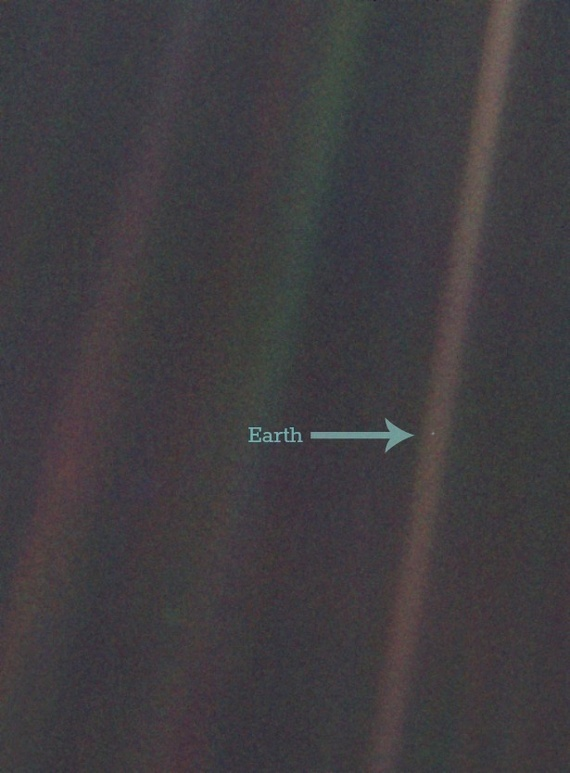
\includegraphics[height=0.8\textheight]{pale-blue-dot.jpg}
\end{center}
}


\frame{\frametitle{\textbf{Accommodations for events on campus: final exam}}

The final exam will now consist of two distinct parts:

\BI
\item A standard-length exam on Unit 4, graded as a standard exam
	\BI
\item This can be dropped like any other exam if it is your lowest grade
	\EI
	\BS
\item About a dozen questions on each of the previous units
\item Each of these segments will now be an opportunity to improve your grade on the previous exam
	\BI
\item If you do better on one of these than you did on a previous exam, it will raise your grade on that exam
\item If you do worse, then it won't affect anything
	\EI

	\BS
\item They are all optional; if you want to devote your time to other things, you don't have to take them
	\EI

The exams in the course will, in total, still comprise the same portion of your final grade.
}

\frame{\frametitle{\textbf{Accommodations for events on campus: project}}
\BI
\item If you do not do a final project, its weight will be reallocated among all other components of the course (``dropped'')

\BS

\item This will likely on average be slightly detrimental to your grade, since final project grades tend to run slightly above other things.

	\BS

\item If you do complete a final project, it will likely help you (and, if you do something excellent, possibly help you a great deal). 
	
\BS

\item These projects are often very rewarding for students, and if you have something rewarding you want to do, do it and enjoy, and this will help your grade! 


	\BS

\item But if you are viewing it as "another paper you have to write", you may skip it and we'll calculate your grade from the rest of your work.

\EI
}

\frame{\frametitle{\textbf{Accommodations for events on campus: recording}}
\Large
Class today will be audiorecorded to accommodate students who are not here.
}



\frame{\frametitle{\bf Summary}
\large
\BI
\item Review: the greenhouse effect
\medskip
\item History
\BI
\normalsize
\item What is the history of the Earth's climate?
\item What processes caused it to vary?
\item How do they affect each other? 
\EI
\medskip
\item The Anthropocene: the era of human influence on geology 
\BI
\normalsize
\item In an eyeblink, a drastic jump in atmospheric ${\rm CO}_2$:
\item Evidence that this is already causing warming
\item Evidence that this has the potential to cause far more warming
\EI
\EI
}

\frame{\frametitle{\bf Summary, II}
\large
\BI
\item Consequences
\BI
\normalsize
\item Exaggerated effect in the Arctic
\item Sea level rise
\item Disruption to society
\item Ecological shocks and extinctions
\EI
\medskip
\item What do we do about this?
\BI
\normalsize
\item What are the sources of $\rm CO_2$ emissions?
\item {\it Who} are the sources of $\rm CO_2$ emissions (spoiler: us)
\item Electricity generation 
\item Transportation
\item Obstacles, legitimate and otherwise 
\item Positive signs
\EI
\EI
}

\frame{\frametitle{\bf The greenhouse effect}

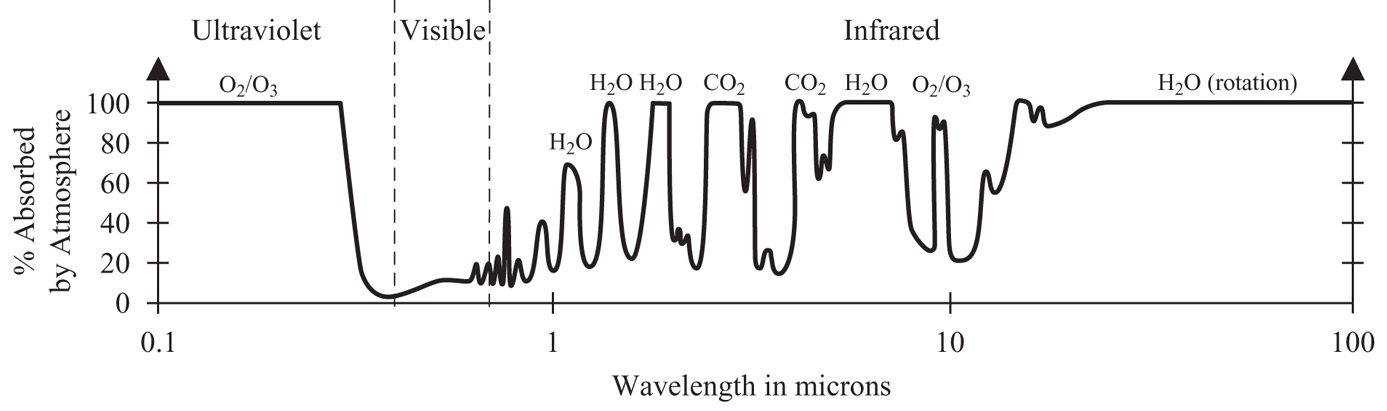
\includegraphics[width=\textwidth]{absorption.jpg}

}

\frame{\frametitle{\bf The greenhouse effect}
Venus has a {\it tremendously thick} atmosphere and a powerful greenhouse effect.

\BI
\item Its atmosphere contains a great deal of $\rm CO_2$, which reflects IR strongly
\item The thermal radiation that would carry heat away from Venus can't get out
\item It is over 400 K hotter than was predicted by the calculation you did last week
\EI

\BS

Earth has a {\it thinner} atmosphere.

\BI
\item Nitrogen doesn't absorb strongly at any relevant wavelengths
\item $\rm H_2 O$ and $\rm CO_2$ are strong greenhouse gases, but they are only a bit of the atmosphere
\item We are about 20 K warmer than predicted by that crude math (more precise math: 30 K)
\item These gases are very important for determining Earth's temperature!
\EI
}

\frame{\frametitle{\bf The greenhouse effect}

The upshot:

\large 

\BI
\item The Sun is around 5500 K, and emits visible/short-wavelength IR; this goes through Earth's atmosphere and warms it
\item The Earth is around 300K K, and emits longer-wavelength IR
\item Some of that energy is absorbed by gases (water, carbon dioxide, methane) in the atmosphere
\item When the atmosphere reradiates it, much of it falls back to Earth
\item {\color{Red} If the short-wavelength sunlight has an easier time getting in than the long-wavelength Earthlight has getting out, Earth's temperature will go up}
\item This is called the {\color{Green}greenhouse effect}.
\EI
}

\frame{\frametitle{\bf Variation of Earth's climate}
\BC
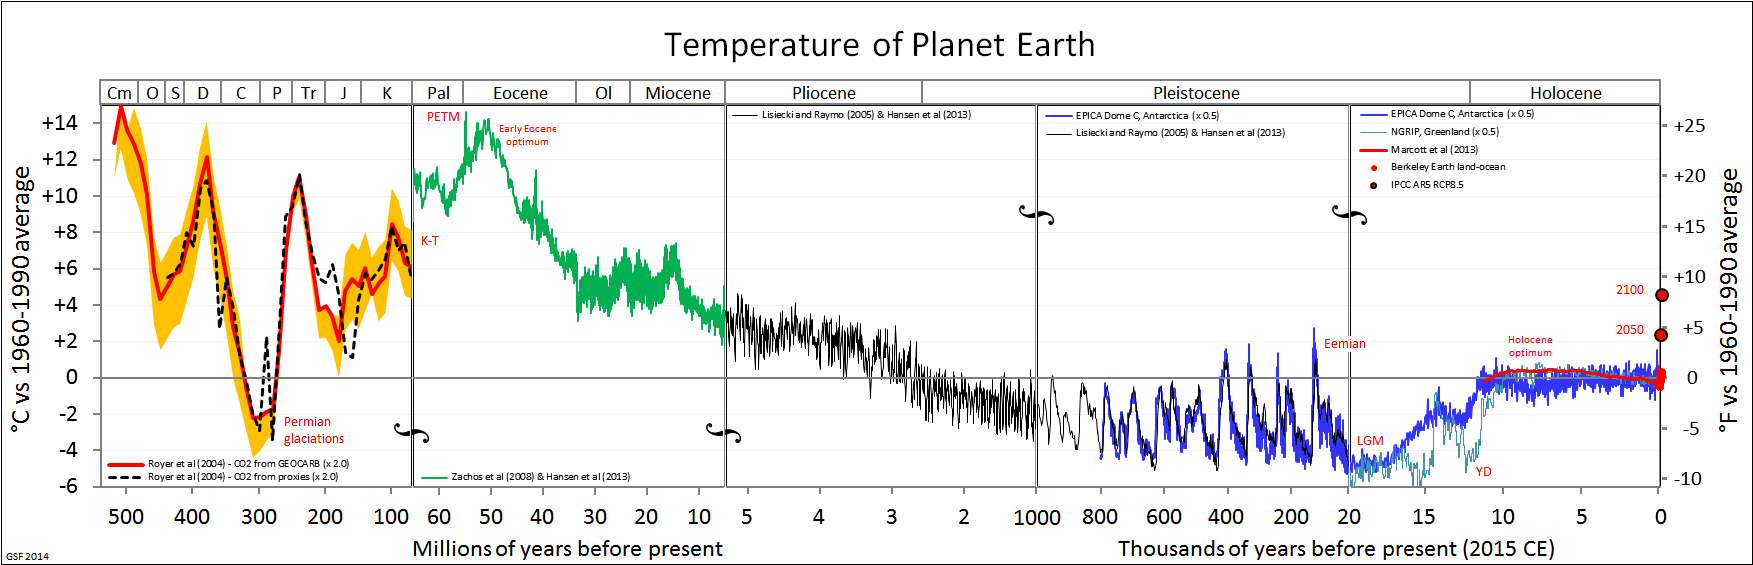
\includegraphics[width=\textwidth]{palaeotemps.png}

\BS\large

Earth has seen quite a lot in its lifetime...

\BS

The past state of Earth can help us study what the future may hold.
\EC
}
\frame{\frametitle{\bf The climate spectrum}

\large
Temperature differences compared to 20th century average:
\BS
\BI
\item -33C: complete lack of greenhouse effect
\item -10C: ``snowball Earth''; glaciers cover entire planet except for a small band at Equator
\item -5C: ice age; Syracuse covered in glaciers
\item 0C: our familiar climate
\item +5C: ??? (but maybe our future)
\item +10C: Like the time of the dinosaurs; inland seas common; much of America underwater
\EI
}


\frame{
\large
What process is most driving these fluctuations in climate?

\BS

\color{A}A: Changes in the Sun's brightness affect the amount of energy reaching Earth\\\BS
\color{B}B: Changes in the rate that volcanoes discharge greenhouse gases into the atmosphere affect the strength of the greenhouse effect\\\BS
\color{C}C: Changes in the Earth's orbit affect the axial tilt and the distance from the Sun\\\BS
\color{D}D: All of the above\\\BS
\color{E}E: An increase in $\rm CO_2$ in the atmosphere due to the burning of fossil fuels has increased the strength of the greenhouse effect
}

\frame{
\Large

\BI
\item {\color{A}Solar output:} fluctuates in an 11-year cycle, but creates only an 0.2-degree change
\pause\BS
\item {\color{B}Volcanism:} variation in the amount of greenhouse gases discharged over this timescale is not that large
\pause\BS
\item {\color{C}The ice ages come in cycles...}
\BI
\item This is from cyclical changes in Earth's orbit and tilt, and is what caused the
series of ice ages
\EI 
\pause\BS
\item Look at the time axis -- {\color{D}the industrial revolution} is just the last eyeblink of history\EI
}

\frame{\frametitle{\textbf{Positive and negative feedback}}

\large

The Earth is quite complex. If the Earth warms, then...

\BI
\item ... certain effects will cause even more warming: {\it positive feedback}
\item ... other effects will slow that warming down: {\it negative feedback}
\EI

\begin{columns}

\column{0.5\textwidth}
\BC
\large
{\color{Red}Positive feedback: snow}
\BS

\small
White snow absorbs less heat than dark soil

This is why snow piles take so long to melt!

\BS

This feedback loop is {\it fast} -- it doesn't take that long to melt snow (years)

\EC
\column{0.5\textwidth}
\BC
\large
{\color{cyan}Negative feedback: oceans}
\BS

\small
More $\rm CO_2$ in the air $\rightarrow$ oceans absorb faster

This brings the $\rm CO_2$ levels back down.

\BS

This feedback loop is {\it slow} -- it takes a long time for $CO_2$ to be absorbed (hundreds/thousands of years)
\EC
\end{columns}

\BS
\BC
In the short term, the positive feedback mechanisms win out.

This means that {\it small changes to the climate are amplified.}
\EC
}

\frame{
\BC
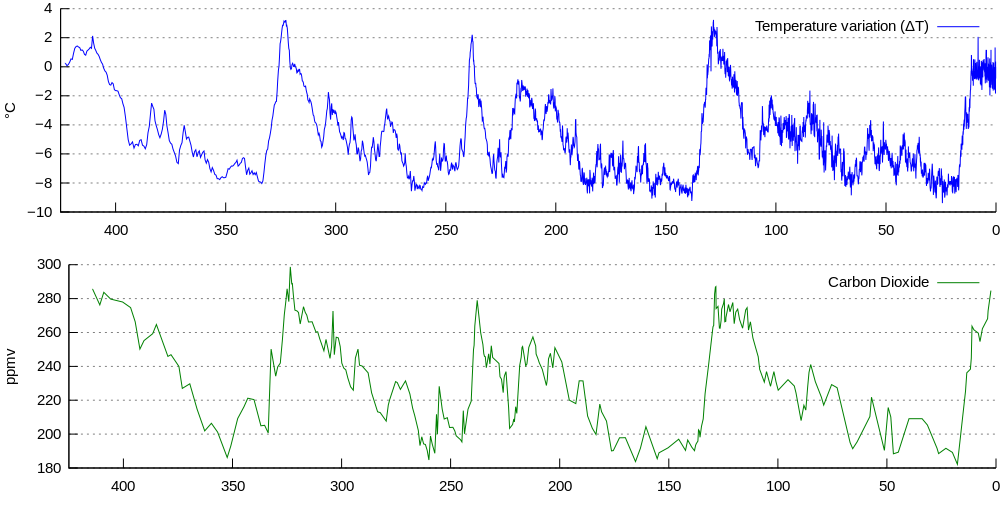
\includegraphics[width=0.95\textwidth]{vostok-petit-co2-temp.png}


$\rm CO_2$ is strongly correlated with temperature (positive feedback).

\BI
\small
\item More $CO_2$ in the atmosphere strengthens the greenhouse effect, raising the temperature
\item Higher temperatures speed up chemical processes that release carbon stored in rocks
\item Lower temperatures speed up chemical processes by which rocks {\it absorb} carbon
\EI


\BS

What if we change $\rm CO_2$ on our own?

\EC

}

\frame{

\Large

What if we change $\rm CO_2$ on our own?

\BS\BS

\color{A}A: The climate will be altered for a few centuries \\\BS
\color{B}B: The climate will be altered for a few tens of thousands of years\\\BS
\color{C}C: The climate will be altered for a few million years\\\BS
\color{D}D: The climate will be altered forever \\\BS

}

\frame{

\Large

How high must atmospheric $\rm CO_2$ levels get for the climate to be seriously changed
compared to the past few hundred thousand years?


\BS\BS

\color{A}A: 275 ppm (parts per million -- see plot)  \\\BS
\color{B}B: 300 ppm \\\BS
\color{C}C: 325 ppm \\\BS
\color{D}D: 350 ppm \\\BS
}

\frame{\frametitle{\bf The current state}
\large
\BC
The 2017 average $\rm CO_2$ level was {\color{Red}405 ppm}.

The Industrial Revolution took us there in a geological blink of an eye.

\BS

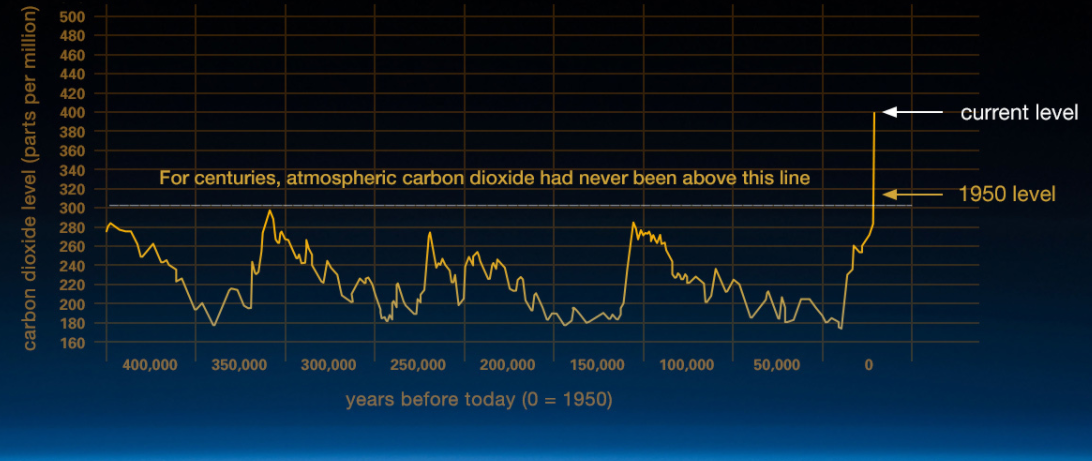
\includegraphics[width=0.95\textwidth]{nasa-co2-hockeystick.png}

\scriptsize \it (NASA)
\EC
}

\frame{\frametitle{\bf The current state}
\large
\BC
The 2017 average $\rm CO_2$ level was {\color{Red}405 ppm}.

The Industrial Revolution took us there in a geological blink of an eye.

\BS

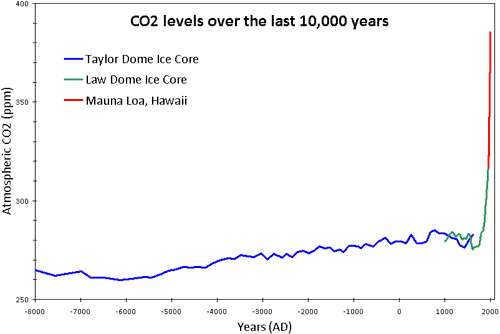
\includegraphics[width=0.7\textwidth]{co2-10k.png}

\EC
}

\frame{\frametitle{\bf What will this do to Earth?}
\Large
\BC
Geophysics is enormously complicated. 

\BS

Models (from simple ones to enormous supercomputer simulations) tell us unequivocally: the $\rm CO_2$ produced by humans will warm the planet.

\BS

But for how much, and for how long, and to what effect?

\BS

We'll talk about those models in a bit, but in the meantime, let's look at history to get an answer.
\EC
}

\frame{\frametitle{\bf This happened once before...}

\large

\BC

The ``Paleocene-Eocene Thermal Maximum'' was a sudden release of carbon dioxide 56 Myr ago.
(We're not sure from where, but we know it happened, by looking at isotope ratios in fossils.)

\BS

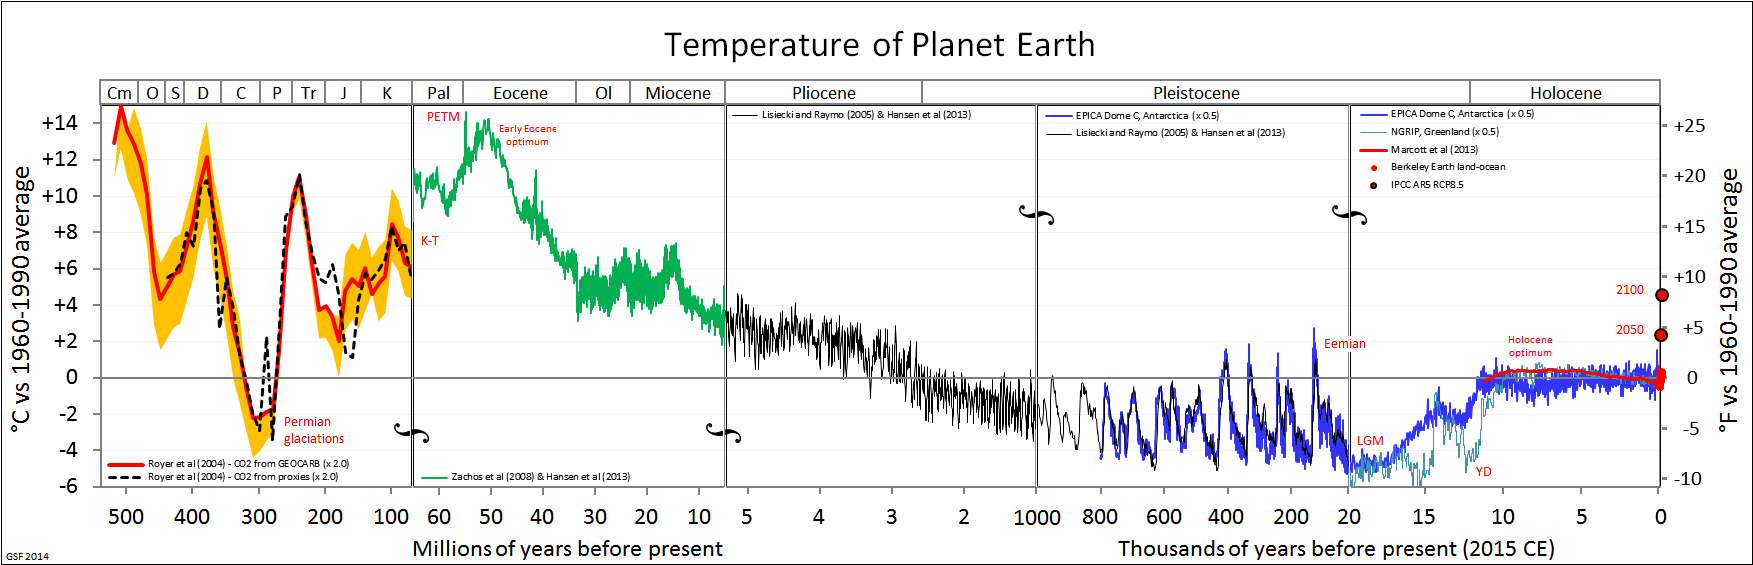
\includegraphics[width=\textwidth]{palaeotemps.png}

\EC

\normalsize
\BI
\item Something caused a rapid release of $\rm CO_2$ over two thousand years, at
      a peak rate of up to 6 billion tons/year.  
\item This caused a temperature spike of 5-8 C that lasted many thousands of years
\item The oceans absorbed much of this carbon as carbonic acid, bleaching corals
\item There was a mass extinction of deep-ocean life and large changes to surface life
\EI
}

\frame{\frametitle{\bf Positive feedback}

\large

Positive feedback effects dominate in the short term: 

\BI
\item Melting of ice, darkening the surface so it absorbs more sunlight
\item Increased amounts of water vapor in the air 
\item Melting of permafrost in Siberia, which has a great deal of trapped methane
\item (Water vapor and methane are also greenhouse gases)
\item $\rightarrow$ Earth processes will magnify any effects from human $\rm CO_2$ emissions
\item \color{Red}Even a little nudge from humans can have large effects
\EI
}

\frame{\frametitle{\bf A candid word on scientific rigor}

As we've discussed, a {\color{Red}crucial} part of scientific integrity is honesty about the limitations of your knowledge. 

\BS

In preparing for this class, I've used as source material:

\BI
\item The UN Intergovernmental Panel on Climate Change Fifth Assessment Report (2015)
\item The US Fourth National Climate Assessment (2017-018)
\EI

\BS

These documents are {\it meticulous} about this. They make sure to describe:

\BI
\item uncertainties in measurements and estimates
\item how confident they are in conclusions
\item when important things are still unknown
\EI

These climate assessments are exemplary in their integrity and honesty in this regard. 

}

\frame{\frametitle{\bf What climate change is and is not}

\large Climate change is a moderate, overall warming of the planet by a few degrees.

\BS

\large It does not mean an end to cold weather -- and cold weather does not mean that
climate change is not happening.

\BS

Most of the world will have more hot extremes and fewer cold ones, but there is a difference
between weather and climate.
}

\frame{\frametitle{\bf Effects on the Arctic}
\large\BC
Computer models and observations show that the 
effects of current and future warming are magnified in the Arctic, because of the albedo effect from melting snow.

\BS

\includegraphics[width=0.8\textwidth]{giss-warming-regions.png}

\BS

\url{https://www.youtube.com/watch?v=VIxciS1B9eo}
\EC
}


%\frame{\frametitle{\bf Effects on the Arctic}
%
%Melting Arctic ice will have catastrophic effects on the Arctic ecosystem, which
%the World Wildlife Fund put bluntly:
%
%\BC
%\includegraphics[width=0.7\textwidth]{chicago-airport-wwf.jpg}\\
%\scriptsize (Photo: Chicago airport terminal, 2016)
%
%\EC
%}


\frame{\frametitle{\bf Sea level rise}
\BC
All that water must go somewhere; heat also causes the oceans to expand.
The Marshall Islands may simply cease to exist.

\BS

\includegraphics[width=0.7\textwidth]{marshall_islands.jpg}

Miami, Manhattan, New Orleans, etc. are also threatened...

\EC

}

\frame{\frametitle{\bf It's definitely happening, and we did it}
\normalsize
{\it Global climate is changing rapidly compared to the pace of natural variations in climate that have occurred throughout Earth’s history. Global average temperature has increased by about $1.8^\circ$ F from 1901 to 2016, and observational evidence does not support any credible natural explanations for this amount of warming; instead, the evidence consistently points to human activities, especially emissions of greenhouse or heat-trapping gases, as the dominant cause.}

\begin{flushright}
\BS\BS--The Fourth National Climate Assessment (US Government), 2018
\end{flushright}

\BS\BS\pause

}



\frame{\frametitle{\bf A word on computer modeling}
\BCC
\HC
\includegraphics[height=0.9\textheight]{climate-simulations.png}
\HC
We've gone from the simple calculations of Arrhenius to massive supercomputer simulations of the Earth's climate.

\BS

If we're going to trust them to predict details about the future, they ought to accurately capture the past.

\BS
\BS

The observed climate trends {\it are not} consistent with simulations of natural influences on the climate, but 
are {\it very} consistent with simulations including human effects.

\BS
\BS

{\color{Red}Climate simulations are accurate for broad trends like global temperature.}
\ECC
}



%\frame{\frametitle{\bf What about the future?}
%\BC
%The main driver of long-term climate effects is the {\color{Red}cumulative amount of $\rm CO_2$} released by humans.
%\EC
%\HC
%\BC
%
%
%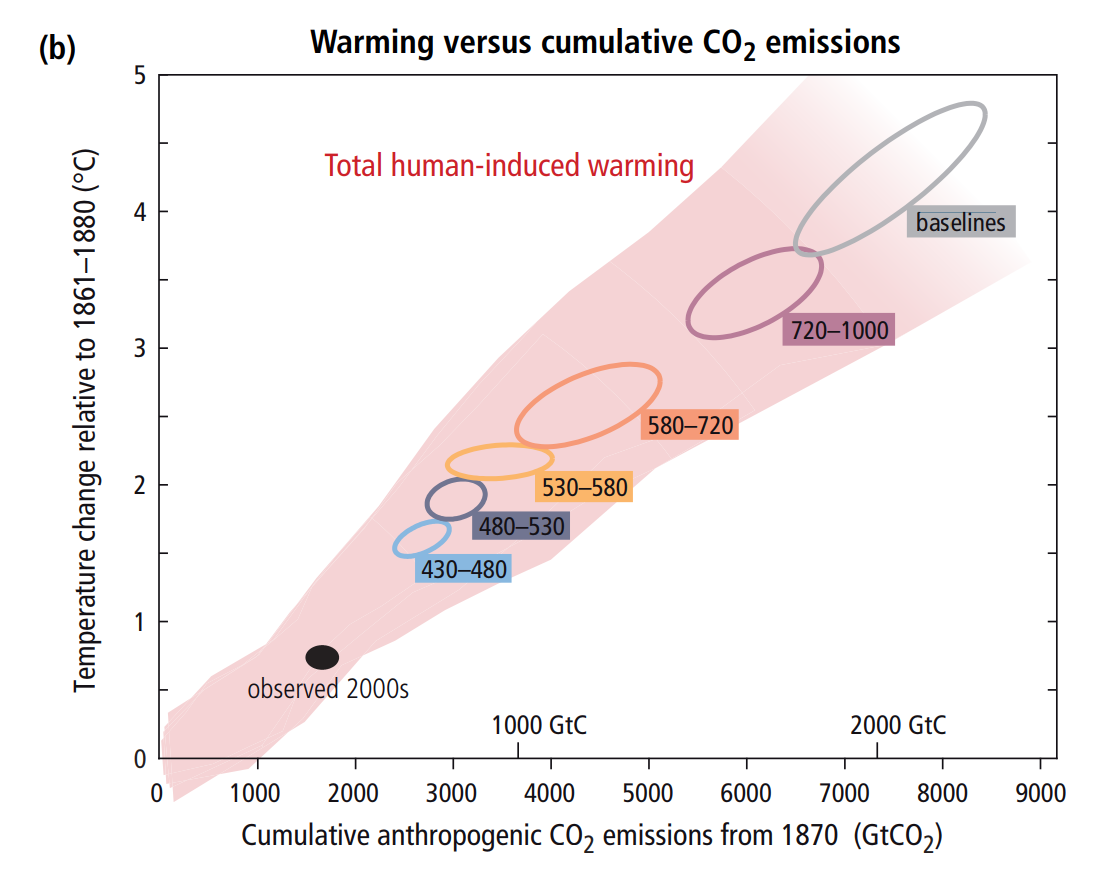
\includegraphics[width=\textwidth]{cumulative-emission-scenarios.png}
%
%\EC
%
%\HC
%
%{\it [T]he evidence of human-caused climate change is overwhelming and continues to strengthen... and climate-related threats to Americans' physical, social, and economic well-being are rising. These impacts are projected to intensify--{\color{Red}but how much they intensify will depend on actions taken to reduce global greenhouse gas emissions and to adapt to the risks from climate change now and in the coming decades.}}
%\begin{flushright}--US FNCA\end{flushright}
%
%\BS\BS\BS
%
%Some warming is inevitable -- but how much more depends on our choices.
%}
%%
%%\frame{\frametitle{\bf Other ecological effects}
%\BC
%Where is this?
%\EC
%
%\BS
%
%\begin{columns}
%\column{0.7\textwidth}
%\includegraphics[width=0.9\textwidth]{wrightson1024.jpg}
%\column{0.3\textwidth}
%
%\color{A}A: the Canadian Rockies\\\BS 
%\color{B}B: the Southern Arizona desert\\\BS
%\color{C}C: near Denali, in Alaska\\\BS
%\color{D}D: the Adirondacks, in NY 
%\end{columns}
%}
%

\frame{\frametitle{\bf Effects on humans}
\large
Our societies are adapted for certain weather patterns and coastlines. If the earth warms:

\BI
\item People may have to abandon coastal cities like Manhattan and Miami
\pause
\item Overall warming will render a lot of land unfarmable in Africa
\pause
\item Seasonal rainfall patterns that equatorial farmers rely on may change
\pause
\item Extreme weather events may become more likely, including wildfires and storms
\EI


\BS

In wealthy nations like the US this will cause massive economic losses, as people are forced to adapt.

\BS

In poorer nations people may not have the resources to adapt...

}

\frame{\frametitle{\bf Climate change mitigation}
\BCC
\column{0.6\textwidth}
The effect on global temperature -- and on human society -- will depend a great deal on {\color{Red}how quickly and deeply we cut $\rm CO_2$ emissions.}
\BI
\small
\item Warming to date: $1^\circ$ C ($2^\circ$ F)
\item Depending on our choices: from $2-7^\circ$ C ($4-12^\circ$ F likely.
\item The next decade or two are crucial for what happens later
\EI
\BC
\includegraphics[width=0.6\textwidth]{obama-climate-change-1.png}
\EC
\column{0.4\textwidth}
\BC
\vspace{-0.5in}
\includegraphics[width=0.9\textwidth]{emissions-scenarios.png}\\
\includegraphics[width=0.8\textwidth]{emissions-damage-2.png}
\EC
\ECC

}

\frame{\frametitle{\bf What's going on now?}
\BC
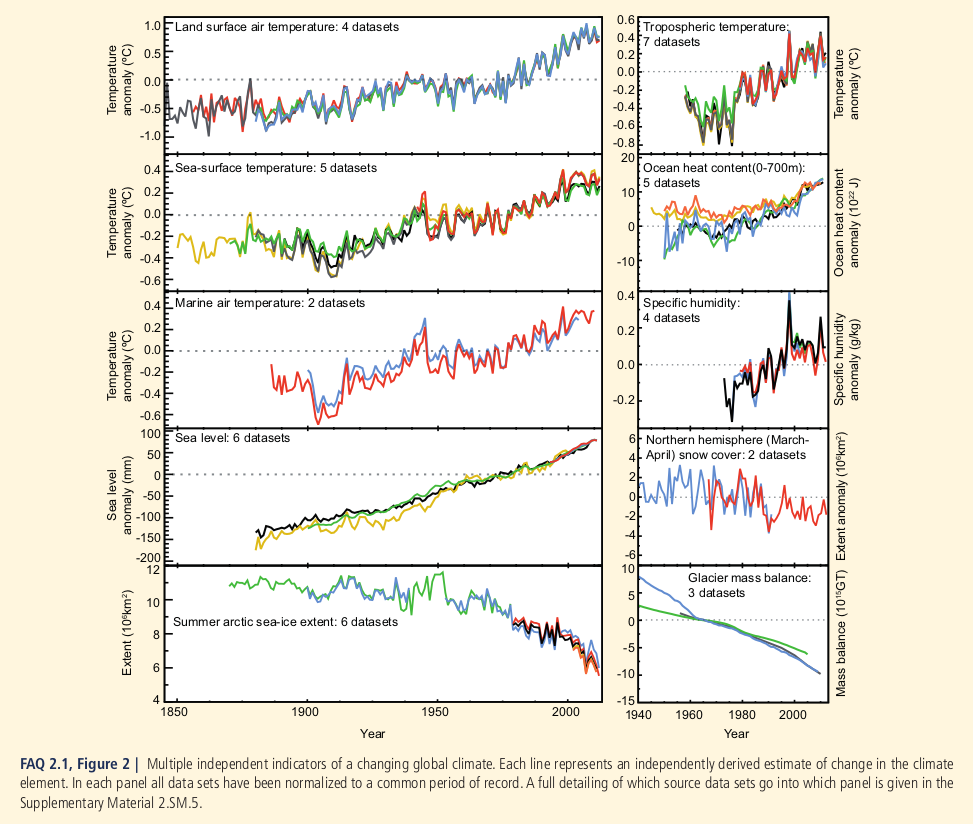
\includegraphics[width=0.72\textwidth]{ipcc-warming-evidence.png}\\
\scriptsize \it (IPCC FAR)
\EC
}




\frame{\frametitle{\bf Sources of $\rm CO_2$ emissions}

\BC
\includegraphics[width=0.9\textwidth]{ipcc-ghg-share.png}

Most of our greenhouse gases come from burning fossil fuels.

\BS

These are mostly used to generate electricity, power vehicles, and in industry.

\EC
}

\frame{\frametitle{\bf Who's doing most of this?}

\large Us -- the global wealthy.

\BS
\BC
\includegraphics[width=0.5\textwidth]{emissions-by-country.jpg}\\
\scriptsize (from the Union of Concerned Scientists)
\EC

%\small
%\url{http://data.worldbank.org/indicator/EN.ATM.CO2E.PC?view=map&year=2013} \\
%\url{http://bit.ly/2gEgkTM} (gapminder.org)
}

\frame{\frametitle{\bf Top $\rm CO_2$ sources}
\BC
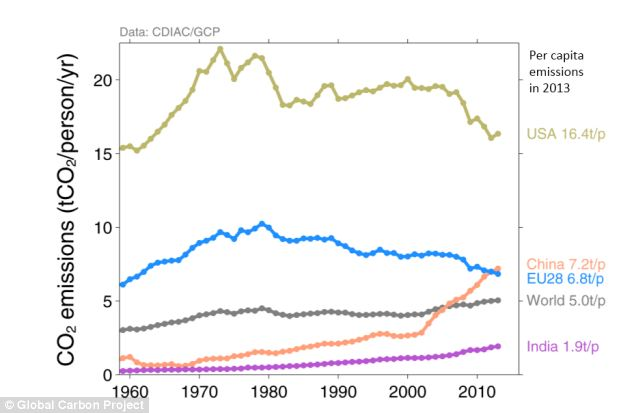
\includegraphics[width=0.8\textwidth]{top-emitters.jpg}

\BS
\large What do you conclude from these data?
\EC
}

\frame{\frametitle{\bf Pointing fingers}
\large
Globalization means that countries now specialize in different things:

\BI
\item Many wealthy countries (USA, France) are moving away from industrial economies (``Rust Belt'')
\item Middle-income countries are industrializing, with many of their products exported
\pause
\item It is wrong to only blame industrial countries like China for $\rm CO_2$ emissions -- this misses a big part of the story
\item My laptop: designed by Americans, CPU by Americans and Israelis, software from a South African company, built in China with {\color{Red} Chinese aluminum}
\item ... but used by an American!
\item \color{Red} In a global economy, this is a global problem!
\EI
}


\frame{\frametitle{\bf A crossroads}
\large
\BC
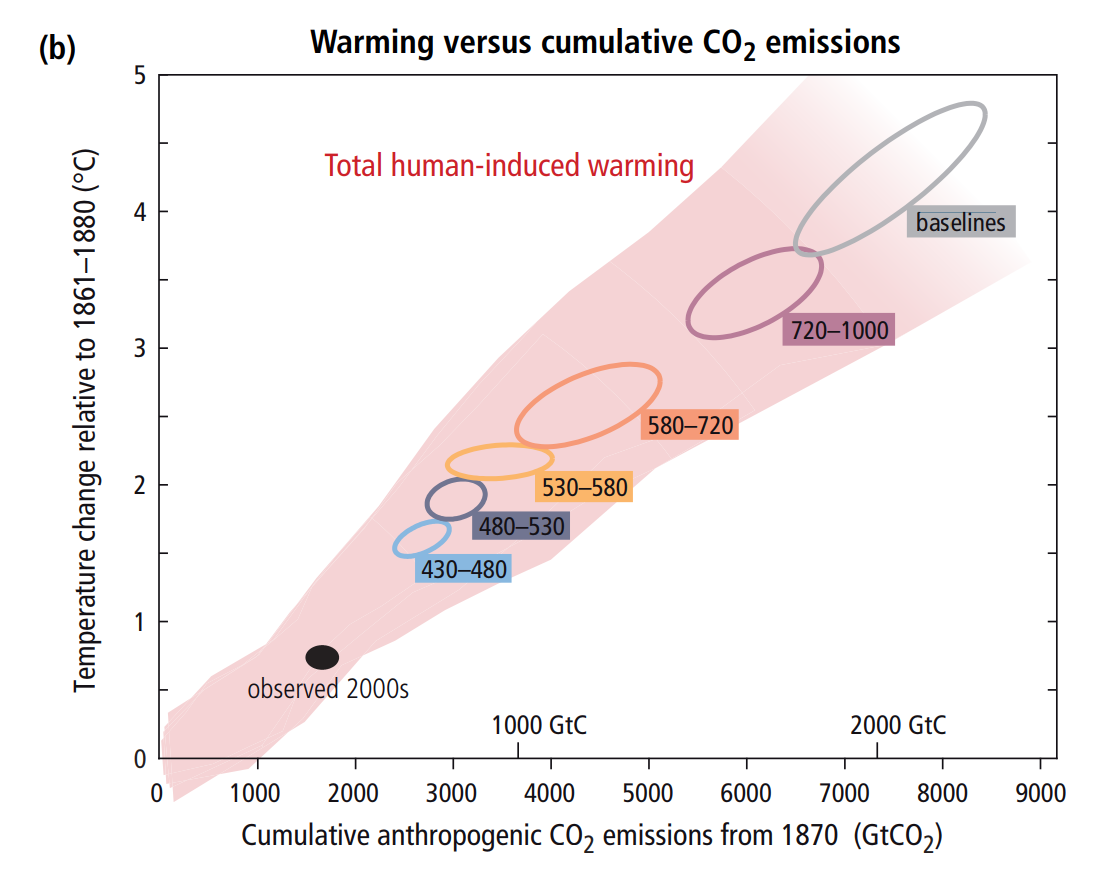
\includegraphics[width=0.6\textwidth]{cumulative-emission-scenarios.png}

\BS
Warming is inevitable (it's already happened). How much more depends on our choices.
\EC
}



\frame{\frametitle{\bf Electricity generation}
\large
Electrical power is the largest source of $\rm CO_2$ emissions.

\BI
\item Coal: cheap and easy, but emits lots of $\rm CO_2$
\item Natural gas: Rapidly becoming cheap (fracking), and emits roughly half the $\rm CO_2$
\EI

\BS
\pause
\Large

Should we invest in natural gas power plants? 

\large\BS

\color{A}A: Yes; they emit less $\rm CO_2$ for the energy we get \\\bigskip
\color{B}B: No; we should only build zero-emissions power plants \\\bigskip
\color{C}C: Yes; American energy independence is important and we have lots of gas \\\BS
\color{D}D: No; once built the gas industry will politicize their continued use 

}

\frame{\frametitle{\bf Electricity generation}
\large
Electrical power is the largest source of $\rm CO_2$ emissions.

\BI
\item Coal: cheap and easy, but emits lots of $\rm CO_2$
\item Natural gas: Rapidly becoming cheap (fracking), and emits roughly half the $\rm CO_2$
\EI

\BS
Zero-emissions power sources:
\BI
\item Hydropower: Cheap, but not always available, and disrupts rivers
\item Nuclear: Large startup cost, more expensive than coal/gas, but reliable and clean
\item Geothermal: Cheap where you've got it; clean
\item Wind: More expensive and fickle
\item Solar: {\it Rapidly} decreasing in cost 
\EI
}

\frame{
\BC
\includegraphics[width=0.8\textwidth]{cost-by-source.png}\\
\scriptsize (Wikipedia / US Energy Information Administration)
\EC

\BS
\large	
Costs vary greatly based on location and other factors!
}

\frame{\frametitle{\bf Transportation}
\large
\BI
\item Cars -- prices dropping, charging infrastructure growing rapidly
\item Buses -- great in cities (see ``bus rapid transit'')
\item Trains -- great if you have the transport density
\item Bicycles -- the most efficient transport in existence
\item Airplanes -- long-distance fast travel is very hard
\EI

\BS
Steps forward:
\BI 
\item Continual gains in efficiency: smaller/better cars, hybrid cars/buses
\item Electrification of everything we can: electric trains, electric cars/lorries
\item Improve mass transit access and desirability
\item Bike lanes in cities
\item Rail/air balance for long-haul travel is hard
\EI
}


\frame{\frametitle{\bf The ``tragedy of the commons''}
\large The problem:

\BI
\item Carbon emissions consume a {\it shared resource} -- the ability of Earth to absorb them
\item Our economic markets are based on {\it price signals}:
\BI
\item If a resource is precious, limited, or labor-intensive, its owner will charge more for it
\item People will buy less of it since it costs more
\EI
\item ... the atmosphere is shared by everyone, but it's hard to assert ``ownership'' of 
\item There is currently no charge at {\it all} for using that resource!
\EI
}

\frame{\frametitle{\bf On politics (warning: personal opinion!)}
\Large
\BC
Climate action in the USA is often framed as a partisan issue.

\BS

But it doesn't need to be a {\it politically divisive} issue!

\BS

There are liberal, conservative, socialist, and libertarian framings of both the problem of climate change and its solutions.
\EC
}


\frame{\frametitle{\bf Avenues for climate change mitigation}

\BI
\item Ban things like coal or very inefficient cars: simple, but a sledgehammer
\medskip
\pause
\item ``Cap and trade'': need a permit to burn fossil fuels. Society decides to what extent
to limit $\rm CO_2$ and auctions that many permits; market forces determine how best to
use them
\medskip
\item Carbon fee: Similar idea, where market incentives raise the cost and thus decrease the use of fossil fuels
\item Government subsidies for lower-emission alternatives
\item Decarbonization of the public sector
\EI
}

\frame{\frametitle{\bf Balance between rich and poor countries}
India and China have built a lot of coal power plants.

\BS

Some arguments:

\BI
\item ``It's not fair for developed countries to have burned their coal already, but developing countries can't benefit in the same way, just because they were a little later''
\item ``Things are different now that we know what $\rm CO_2$ does, so developing countries
are going to have to leave their coal in the ground''
\pause\BS
\item Idea of ``climate debt'': the West owes poor countries payment for their cumulative
past emissions, and help with GDP growth in a low-carbon economy
\pause\BS
\item \color{Red} We're all in this together -- global problems demand global action
\EI
}

\frame{\frametitle{\bf Obstacles}
\BI
  \item ``Regulatory capture'' of government by fossil fuel industry
  \item Organized campaign of misinformation (compare to smoking/cancer link)
  \item Manufactured controversy:
  \BI
    \item The overwhelming scientific consensus stands behind what I've presented
    \item ... but well-funded ``skeptics'' can speak with a loud voice
  \EI
  \BS
  \item Distraction:
  \BI
    \item Eyes have lately been (rightfully) drawn to other issues in politics 
\item This is a hard time to think about decades-long issues...
\EI
\BS
\item International nature of the problem:
\BI
\item Addressing climate change requires cooperation between nations
\item Our species has never really done this before
\item Historical asymmetry between nations
\EI
\EI
}

\frame{\frametitle{\bf Summary}
\BI
\item Carbon dioxide level in the atmosphere acts as a ``thermostat'' for Earth
\item $\rm CO_2$ from human fossil fuel use is raising that level
\pause
\BS
\item The climate is getting warmer and will continue to get warmer:
\BI
\item $1^\circ$C warming already
\item $2-7^\circ$C warming likely in a hundred years
\item Future $\rm CO_2$ emissions will determine where in that range
\EI
\item These changes are on the same level as natural variations of Earth's climate

\pause\BS

\item ... but they are happening far faster. This has already caused issues:
\BI
\item More / more intense hurricanes
\item More / more intense wildfires
\item Sea level rise 
\item Altered rainfall patterns
\EI
\item Future issues are likely to be a lot worse

\pause
\BS

\item Solutions are technically well-understood
\item ... the problem is just the cooperation needed to implement them
\EI
}




\end{document}
